\documentclass[margin,line]{res}
\usepackage{hyperref}
\usepackage{pifont}
\usepackage[latin1]{inputenc}
\usepackage{longtable}
%\topmargin .5in
%\oddsidemargin -.5in
%\evensidemargin -.5in
%\textwidth=6.0in
\textheight=9.0in
%\itemsep=0in
%\parsep=0in
\usepackage{fancyhdr}
\topmargin=-.25in
%\textheight=8.5in
\pagestyle{fancy}
\renewcommand{\headrulewidth}{0pt}
\fancyhf{}

\usepackage{graphicx}
\usepackage{changepage} 
\usepackage{enumitem}


%\cfoot{\thepage}
%\lfoot{\textit{\footnotesize Research Statement}}
%\rfoot{{\footnotesize Curriculum Vitae, Justin C. Bagley, \thepage}}
\rfoot{{\footnotesize Justin C. Bagley \textendash~CV \thepage}}

%%%% NAME

\begin{document}
\name{Justin C. Bagley \vspace*{.1in}}
\begin{resume}


%%%% CONTACT INFORMATION

\section{\sc Contact Information}
\vspace{.05in}
\begin{tabular}{@{}p{2.75in}p{2in}}
\href{http://www.jsu.edu/biology/}{Department of Biology} & Phone: (256) 782-8641 \\
\href{http://www.jsu.edu}{Jacksonville State University} & Office: ~(256) 782-5642 \\
242 Martin Hall, 700 Pelham Rd N & E-mail: \href{mailto:jbagley@jsu.edu}{\tt jbagley@jsu.edu} \\
Jacksonville, AL 36265, USA & Website: \href{https://justinbagley.org/}{\tt https://justinbagley.org/} 
%\href{http://umsl.edu/\%7Ebiology/index.html}{University of Missouri\textendash St. Louis} & (314)-516-5125 (office)\\
%\href{mailto:bagleyj@umsl.edu}{bagleyj@umsl.edu} & \href{https://justinbagley.org}{https://justinbagley.org}\\
\end{tabular}


%%%% ACADEMIC POSITIONS (FILL IN WITH PROFESSORSHIPS)

%% example text/formatting:
%\section{\sc Academic Positions}
%{\bf \href{http://www.ucsd.edu/}{University of California, San Diego}}\\
%\vspace*{-.1in}
%\begin{itemize}
%\item[] \hspace*{-2mm} \textit{Assistant Teaching Professor}, %\href{http://www.cs.ucsd.edu/}{Computer Science \& Engineering} (2019 -- Present)
%\begin{itemize}
%\item Affiliation: \href{http://bioinformatics.ucsd.edu/}{Bioinformatics and Systems Biology Graduate Program}
%\item Affiliation: \href{http://dbmi.ucsd.edu/}{Department of Biomedical Informatics (School of Medicine)}
%\item Affiliation: \href{https://datascience.ucsd.edu/research/life-cluster/}{Hal{\i}c{\i}o{\u g}lu Data Science Institute}
%\end{itemize}
%\end{itemize}


%%%% PROFESSIONAL APPOINTMENTS (POST-PHD ACADEMIC EMPLOYMENT)

\section{\sc Professional Appointments}
{\bf \href{http://www.jsu.edu/}{Jacksonville State University}}, Jacksonville, Alabama, USA\\
\vspace*{-.1in}
\begin{itemize}
\item[] \hspace*{-2mm} \textit{Assistant Professor}, Department of Biology  (2020 -- present)
\end{itemize}
\vspace*{-.1in}
{\bf \href{http://www.umsl.edu/}{University of Missouri\textendash St. Louis}}, St. Louis, Missouri, USA\\
\vspace*{-.1in}
\begin{itemize}
\item[] \hspace*{-2mm} \textit{Postdoctoral Research Associate}, Department of Biology  (2018 -- 2020)
\begin{itemize}
\item Advisor: Nathan Muchhala (Funding: \href{https://www.nsf.gov/awardsearch/showAward?AWD_ID=1754802&HistoricalAwards=false}{NSF DEB})
\end{itemize}
\end{itemize}
\vspace*{-.1in}
{\bf \href{https://www.vcu.edu/}{Virginia Commonwealth University}}, Richmond, Virginia, USA\\
\vspace*{-.1in}
\begin{itemize}
\item[] \hspace*{-2mm} \textit{Affiliate Researcher}, Department of Biology  (2018 -- present)
\item[] \hspace*{-2mm} \textit{Postdoctoral Scholar}, Department of Biology  (2017 -- 2018)
\begin{itemize}
	\item Advisor: Andrew J. Eckert (Funding: \href{https://www.nsf.gov/funding/pgm_summ.jsp?pims_id=503425}{NSF Macrosystems Biology})
\end{itemize}
\end{itemize}
\vspace*{-.1in}
{\bf \href{https://www.unb.br/}{Universidade de Bras\'{i}lia}}, Bras\'{i}lia, Distrito Federal, Brazil
%\vspace*{-.1in}
\begin{itemize}
	\item[] \hspace*{-2mm} \textit{Senior Research Associate}, Departamento de Zoologia  (2015 -- 2018)
\end{itemize}
%\vspace*{-.1in}
{\bf \href{https://www2.unesp.br/}{Universidade Estadual Paulista (UNESP)}}, S\~{a}o Jose do Rio Preto, S\~{a}o Paulo, Brazil
%\vspace*{-.1in}
\begin{itemize}
	\item[] \hspace*{-2mm} \textit{Young Talent Fellow Postdoc}, Departamento de Zoologia e Bot\^{a}nica  (2015 -- 2017)
\begin{itemize}
%	\item Director: Francisco Langeani; Coordinator: Guarino R. Colli (Funding: Science Without Borders program, Conselho Nacional de Desenvolvimento Cient\'{i}fico e Tecnol\'{o}gico (CNPq))
%	\item Director: Francisco Langeani; Coordinator: Guarino R. Colli (Funding: Science Without Borders, CNPq, Brazil)
	\item Director: Kiko Langeani; Coordinator: Guarino R. Colli (Funding: \href{http://www.cnpq.br/}{CNPq})
\end{itemize}
\end{itemize}
\vspace*{-.1in}
{\bf \href{https://www.uvu.edu}{Utah Valley University}}, Orem, Utah, USA
%\vspace*{-.1in}
\begin{itemize}
	\item[] \hspace*{-2mm} \textit{Adjunct Instructor of Ecology}, Department of Biology  (Summer 2014)
\end{itemize}


%%%% EDUCATION

\section{\sc Education}
{\bf \href{https://www.byu.edu/}{Brigham Young University}}, Provo, Utah, USA\\
\vspace*{-.1in}
\begin{itemize}
\item[] \hspace*{-2mm}\href{https://biology.byu.edu/}{Ph.D. in Integrative Biology} (December 2014) %GPA: 3.58
\begin{itemize}
	\item Advisor: \href{https://lifesciences.byu.edu/directory/jerald-johnson/}{Jerald B. Johnson}
\end{itemize}
\end{itemize}
\vspace*{-.1in}
{\bf \href{https://www.ua.edu/}{The University of Alabama}}, Tuscaloosa, Alabama, USA\\
\vspace*{-.1in}
\begin{itemize}
\item[] \hspace*{-2mm}\href{https://bsc.ua.edu}{M.Sc. in Biology} (August 2008) %GPA: 3.39
\begin{itemize}
	\item Advisor: \href{https://bsc.ua.edu/profiles/phillip-m-harris/}{Phillip M. Harris}
\end{itemize}
\item[] \hspace*{-2mm}\href{https://bsc.ua.edu}{B.Sc. in Biology} (December 2004) %GPA: 3.43
\begin{itemize}
	\item Advisor: \href{https://bsc.ua.edu/profiles/stephen-m-secor/}{Stephen M. Secor}
\end{itemize}
\end{itemize}
\vspace*{-.1in}
{\bf \href{https://www.sheltonstate.edu/}{Shelton State Community College}}, Tuscaloosa, Alabama, USA\\
\vspace*{-.1in}
\begin{itemize}
\item[] \hspace*{-2mm}A.S. in General Studies (May 2002) %GPA: 4.00
\end{itemize}


%%%% LANGUAGES

\section{\sc Languages}
\emph{Spoken:} English (native), Spanish (near fluent, 9 yrs), Portuguese (functional, 2.5 yrs) \\
\emph{Programming \& Markup:} \textsf{bash}/shell, \href{https://cran.r-project.org}{\textsf{R}}, \href{https://www.python.org}{Python}, \href{https://git-scm.com}{\textsf{git}}, Swift, \href{https://www.markdownguide.org}{Markdown}, \href{https://www.latex-project.org}{\LaTeX}


%%%% RESEARCH INTERESTS

\section{\sc Research Interests}
phylogeography, phylogenomics, population genomics, speciation, adaptation, \\
gene flow (hybridization), species delimitation, integrative taxonomy, ecological \\
niche modeling, phylogenetic comparative methods
%\vspace*{-.1in}
%\begin{itemize}
%	\item[] \hspace*{-2mm}<otherItem>
%\end{itemize}


%%%% PUBLICATIONS

\section{\sc Publications}

%%%%%%%%%%%%%%%%%%%% Figure/Image No: 1 starts here %%%%%%%%%%%%%%%%%%%%

\begin{figure}[h]
	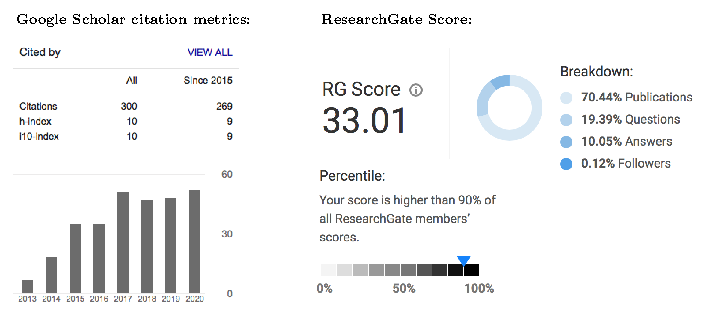
\includegraphics[scale=1.1]{./metrics_Oct152020.pdf}
	%	\centering
\end{figure}

%%%%%%%%%%%%%%%%%%%% Figure/Image No: 1 Ends here %%%%%%%%%%%%%%%%%%%%

\emph{Abbreviations:} \textsuperscript{U}undergraduate student, \textsuperscript{G}graduate student

\textbf{A. Peer-reviewed Journal Papers and Book Chapters}\vspace{2mm}\\*
%25. Calder\'{o}n-Acevedo CA\textsuperscript{G}, \textbf{Bagley JC}, Muchhala N (\textit{in review}). Genome-wide ultraconserved elements resolve phylogenetic relationships, species boundaries, and hybridization among Neotropical leaf-nosed bats in the genus \emph{Anoura} Gray 1838. \textit{\textbf{Molecular Phylogenetics and Evolution}}. \\
%~\\
%24. \textbf{Bagley JC}, Moon S\textsuperscript{U}, Grasso ZG\textsuperscript{U} (\textit{in review}). Phylogeography and diversification in lower Central America: an updated synthesis. In: Neotropical Diversification. (eds Rull V, Carnaval A). \textit{\textbf{Springer}}. \\
%~\\
%23. \textbf{Bagley JC}, Aquino PPU, Hrbek T, Hernandez S\textsuperscript{G}, Langeani F, Colli GR (\emph{in}\\
%\hspace*{8mm} \emph{revision}) Using ddRAD-seq phylogeography to test for genetic effects of \\
%\hspace*{8mm} headwater river capture in suckermouth armored catfish (Loricariidae:\\ \vspace{2mm}
%\hspace*{8mm}\emph{Hypostomus}) from the central Brazilian Shield. {\it \textbf{Molecular Ecology}}.\\%*\vspace{2mm}
%~\\
%
%Soares, Y.F.F., Aquino, P.P.U., Bagley, J.C., Langeani, F., Colli, G.R., in review. Two new species of Hypostomus suckermouth armored catfishes (Teleostei: Loricariidae) from Central Brazil. Journal of Fish Biology.
%
22. Soares YFF, Aquino PPU, \textbf{Bagley JC}, Langeani F, Colli GR (\emph{in review}) Two\\
\hspace*{8mm} new species of \emph{Hypostomus} suckermouth armored catfishes (Teleostei:\\
\vspace{2mm}
\hspace*{8mm} Loricariidae) from Central Brazil. {\it \textbf{Journal of Fish Biology}}. \\
%~\\
21. Menon M, \textbf{Bagley JC}, Page G, Whipple AV, Schoettle AW, Still C, Wehenkel\\
\hspace*{8mm} C, Waring K, Flores-Renteria L, Cushman SA, Eckert AJ (\emph{in press}) Adaptive\\
\hspace*{8mm} evolution in a conifer hybrid zone is driven by a mosaic of introgressed and\\ \vspace{2mm}
\hspace*{8mm}standing genetic variants. {\it \textbf{Communications Biology}}. \\
%~\\
20. \textbf{Bagley JC}, Heming NM, Guti\'{e}rrez EE, Devisetty UK, Mock KE, Eckert AJ,\\
\hspace*{8mm} Strauss SH (2020) Genotyping-by-sequencing and ecological niche \\
\hspace*{8mm} modeling illuminate phylogeography, admixture, and Pleistocene range dynamics\\ \vspace{2mm}
\hspace*{8mm}in quaking aspen (\textit{Populus tremuloides}). {\it \textbf{Ecology and Evolution}}, 10, 4609\textendash 4629.\\
%~\\
19. \textbf{Bagley JC}, Uribe-Convers S, Carlsen M, Muchhala N (2020) Utility of\\
\hspace*{8mm} targeted sequence capture for phylogenomics in rapid, recent angiosperm radia-\\
\hspace*{8mm} tions: Neotropical \emph{Burmeistera} bellflowers as a case study. \textit{\textbf{Molecular Phylo-}\\ 
\hspace*{8mm}\textbf{ genetics and Evolution}}, 152, 106769. Available online. 
\href{doi:10.1016/j.ympev.2020.106769}{\tt doi:10.1016/j.ympev.}\\
\vspace{2mm}
\hspace*{7mm} \href{doi:10.1016/j.ympev.2020.106769}{\tt2020.106769}.\\
%~\\
18. \textbf{Bagley JC}, Aquino PPU, Breitman MF, Langeani F, Colli GR (2019) DNA\\
\hspace*{8mm} barcode and minibarcode identification of freshwater fishes from Cerrado head-\\ \vspace{2mm}
\hspace*{8mm}water streams in central Brazil. \textit{\textbf{Journal of Fish Biology}}, 95, 1046\textendash 1060. \\
%~\\
17. Menon M\textsuperscript{G}, Landguth E, S\'{a}enz AL\textsuperscript{G}, \textbf{Bagley JC}, Schoettle A, Wehenkel CA,\\ 
\hspace*{8mm} Cushman S, Waring K, Eckert AJ (2019) Tracing the footprints of a moving \\
\hspace*{8mm} hybrid zone under a demographic history of speciation with gene flow. \textit{\textbf{Evolu-}\\ \vspace{2mm}
\hspace*{8mm}\textbf{tionary Applications}}, 13(1), 195\textendash 209. \\
%Accepted Author Manuscript \href{doi:10.1111/eva.12795}{\tt doi:10.1111/eva.12795}.\\
%~\\
16. \textbf{Bagley JC}, Hickerson MJ, Johnson JB (2018) Testing hypotheses of diversifica-\\
\hspace*{8mm} tion in Panamanian frogs and freshwater fishes using hierarchical approximate\\ \vspace{2mm}
\hspace*{8mm}Bayesian computation with model averaging. {\it \textbf{Diversity}}, 10, 120. \\
%~\\
15. Breitman MF, Domingos FMCB, \textbf{Bagley JC}, Wiederhecker HC, Ferrari TB\textsuperscript{U},\\ 
\hspace*{8mm} Cavalcante VHGL\textsuperscript{G}, et al.\textsuperscript{UG} (2018) A new species of \emph{Enyalius} (Squamata:\\ \vspace{2mm}
\hspace*{8mm}Leiosauridae) endemic to the Brazilian Cerrado. {\it \textbf{Herpetologica}}, 74(4), 355\textendash 369. \\
%~\\
14. \textbf{Bagley JC}, Harris PM, Mayden, RL (2018) Phylogeny and divergence times of\\
\hspace*{8mm} suckers (Cypriniformes: Catostomidae) inferred from Bayesian total-evidence\\ \vspace{2mm}
\hspace*{8mm}analyses of molecules, morphology, and fossils. {\it \textbf{PeerJ}}, 6, e5168. \\ %{\tt https://doi.org/10.7717/peerj.5168}. \\ 
%~\\
13. Menon MG\textsuperscript{G}, \textbf{Bagley JC}, Friedline C, Whipple A, Schoettle A, S\'{a}enz AL\textsuperscript{G},\\ 
\hspace*{8mm} Wehenkel CA, Flores-Renter\'{i}a LH, Sniezko R, Cushman S, Waring K, Eckert\\
\hspace*{8mm} AJ (2018) The role of hybridization during ecological divergence between south-\\
\hspace*{8mm} western white pine, {\it Pinus strobiformis}, and limber pine, {\it P. flexilis}. {\it \textbf{Molecular}\\ \vspace{2mm}
\hspace*{8mm}\textbf{Ecology}}, 27, 1245\textendash 1260. \\ %{doi: 10.1111/mec.14505}. \\
%~\\
12. Overcast I\textsuperscript{G}, \textbf{Bagley JC}, Hickerson, MJ (2017) Strategies for improving approx-\\
\hspace*{8mm} imate Bayesian computation tests for synchronous diversification. {\it \textbf{BMC Evo-}\\ \vspace{2mm}
\hspace*{8mm}\textbf{lutionary Biology}}, 17, 203. \\
%~\\
11. Cer\'{i}aco LM, Guti\'{e}rrez EE, Dubois A, et al.\textsuperscript{UG} (Appendix 1 of \textbf{Supporting Sig-}\\
\hspace*{8mm} \textbf{natories}) (2016) Photography-based taxonomy is inadequate, unnecessary, and\\ \vspace{2mm}
\hspace*{8mm}potentially harmful for biological sciences. {\it \textbf{Zootaxa}}, 4196, 435\textendash 445. \\
%~\\
10. \textbf{Bagley JC}, Matamoros WA, McMahan CD, Tobler M, Chakrabarty P, John-\\
\hspace*{8mm} son JB (2016) Phylogeography and species delimitation in convict cichlids (Ci-\\
\hspace*{8mm} chlidae: \emph{Amatitlania}): implications for taxonomy and Plio\textemdash Pleistocene evolu-\\
\hspace*{8mm} tionary history in Central America. {\it \textbf{Biological Journal of the Linnean So-}\\ \vspace{2mm}
\hspace*{8mm}\textbf{ciety}}, 120(1), 155\textendash 170. \\
%~\\
9. \textbf{Bagley JC}, Alda F, Breitman MF, van den Berghe E, Bermingham E, Johnson\\
\hspace*{8mm} JB (2015) Assessing species boundaries using multilocus species delimitation in \\
\hspace*{8mm} a morphologically conserved group of Neotropical freshwater fishes, the \emph{Poecilia}\\ \vspace{2mm}
\hspace*{8mm} \emph{sphenops} species complex (Poeciliidae). {\it \textbf{PLoS One}}, 10(4), e0121139. \\
%~\\
8. Watson CM, Makowsky R, \textbf{Bagley JC}\textsuperscript{G} (2014) Reproductive mode evolution in\\ 
\hspace*{8mm} lizards revisited: updated analyses examining geographic, climatic and phyloge-\\
\hspace*{8mm} netic effects support the cold-climate hypothesis. {\it \textbf{Journal of Evolutionary}\\ \vspace{2mm}
\hspace*{8mm}\textbf{Biology}}, 27(12), 2767\textendash 2780. \\
%~\\
7. \textbf{Bagley JC}\textsuperscript{G}, Johnson JB (2014b) Testing for shared biogeographic history in the\\
\hspace*{8mm} lower Central American freshwater fish assemblage using comparative phylo-\\
\hspace*{8mm} geography: concerted, independent, or multiple evolutionary responses? {\it \textbf{Ecol-}\\ \vspace{2mm}
\hspace*{8mm}\textbf{ogy and Evolution}}, 4, 1686\textendash 1705. \\
%~\\
6. \textbf{Bagley JC}\textsuperscript{G}, Johnson JB (2014a) Phylogeography of the lower Central American\\
\hspace*{8mm} Neotropics: diversification between two continents and between two seas. {\it \textbf{Bio-}\\ \vspace{2mm}
\hspace*{8mm}\textbf{logical Reviews}}, 89(4), 767\textendash 790. \\
%~\\
5. \textbf{Bagley JC}\textsuperscript{G}, Sandel M, Travis J, Lozano-Vilano M de L, Johnson JB (2013)\\
\hspace*{8mm} Paleoclimatic modeling and phylogeography of least killifish, \emph{Heterandria for-}\\
\hspace*{8mm} \emph{mosa}: insights into Pleistocene expansion-contraction dynamics and evolution-\\
\hspace*{8mm} ary history of North American Coastal Plain freshwater biota. {\it \textbf{BMC Evolut-}\\ \vspace{2mm}
\hspace*{8mm}\textbf{ionary Biology}}, 13, 223. \\
%~\\
4. Unmack PJ, \textbf{Bagley JC}\textsuperscript{G}, Adams MD, Hammer MD, Johnson JB (2012) Molec-\\
\hspace*{8mm} ular phylogeny and phylogeography of the Australian freshwater fish genus \emph{Galax-}\\
\hspace*{8mm} \emph{iella} (Teleostei: Galaxiidae), with an emphasis on dwarf galaxias (\emph{G. pusilla}).\\ \vspace{2mm}
\hspace*{8mm}{\it \textbf{PLoS One}}, 7(6), e38433. \\
%~\\
3. \textbf{Bagley JC}\textsuperscript{G}, Mayden RL, Roe KJ, Holznagel W, Harris PM (2011). Congeneric\\
\hspace*{8mm} phylogeography reveals polyphyly and novel biodiversity within black basses\\
\hspace*{8mm} (Centrarchidae: \emph{Micropterus}). {\it \textbf{Biological Journal of the Linnean Society}},\\ \vspace{2mm}
\hspace*{8mm}104, 346\textendash 363. \\
%~\\
2. Johnson JB, \textbf{Bagley JC}\textsuperscript{G} (2011) Ecological drivers of life-history evolution. In:\\
\hspace*{8mm} Ecology and Evolution of Poeciliid Fishes. (eds Evans JP, Pilastro A, Schlupp\\ \vspace{2mm}
\hspace*{8mm} I), pp. 38\textendash 49. {\it \textbf{University of Chicago Press}}, Chicago, IL. ISBN-10: 0226222748. \\
%~\\
1. Thompson M\textsuperscript{G}, \textbf{Bagley JC}\textsuperscript{G}, Rasco J, Lackey K, Cox M\textsuperscript{G} (2007) The Respiratory\\
\hspace*{8mm} System. In: Biology: The Study of Life (eds Rasco J, Lackey K). {\it \textbf{Kendall/Hunt}\\ 
\hspace*{8mm}\textbf{Publishing}}. ISBN-10: 0757556434. 

%\vspace*{-.2in}
%\subsection*{\textbf{B. Preprints}}
\textbf{B. Preprints}%\vspace{2mm}\\*

3. \textbf{Bagley JC}, Heming NM, Guti\'{e}rrez EE, Devisetty UK, Mock KE, Eckert AJ,\\
\hspace*{8mm} Strauss SH (2018) Genotyping-by-sequencing and ecological niche modeling il-\\
\hspace*{8mm} luminate phylogeography, admixture, and Pleistocene range dynamics in quaking\\
\hspace*{8mm} aspen (\textit{Populus tremuloides}). {\it \textbf{PeerJ Preprints}}.  Available online at: \\ \vspace{2mm}
\hspace*{8mm}\href{https://peerj.com/preprints/27162/}{\tt https://peerj.com/preprints/27162/}. \\
%~\\
2. \textbf{Bagley JC}, Hickerson MJ, Johnson JB (2018) Testing hypotheses of diversi-\\
\hspace*{8mm} fication in Panamanian frogs and freshwater fishes using hierarchical approximate\\
\hspace*{8mm} Bayesian computation with model averaging. {\it \textbf{PeerJ Preprints}}. Available on-\\ \vspace{2mm}
\hspace*{8mm}line at: \href{https://peerj.com/preprints/26623/}{\tt https://peerj.com/preprints/26623/}. \\
%~\\
1. Menon MG\textsuperscript{G}, \textbf{Bagley JC}, Friedline C, Whipple A, Schoettle A, S\'{a}enz AL\textsuperscript{G}, We-\\
\hspace*{8mm} henkel CA, Flores-Renter\'{i}a LH, Sniezko R, Cushman S, Waring K, Eckert AJ\\
\hspace*{8mm} (2017) The role of hybridization during ecological divergence between south-\\
\hspace*{8mm} western white pine, \emph{Pinus strobiformis}, and limber pine, \emph{P. flexilis}. {\it \textbf{bioRxiv}}.\\
\hspace*{8mm} Link: \href{https://www.biorxiv.org/content/early/2017/09/07/185728}{\tt https://www.biorxiv.org/content/early/2017/09/07/185728}.


%\subsection*{\textbf{C. Manuscripts In Preparation}}
\textbf{C. Manuscripts In Preparation}%\vspace{2mm}\\*

3. Calder\'{o}n\textendash Acevedo CA{G}, \textbf{Bagley JC}, Muchhala N (\emph{in prep.}) Genome-wide ul-\\
\hspace*{8mm} traconserved elements resolve phylogenetic relationships among Neotropical leaf-\\
\hspace*{8mm} nosed bats in the genus \emph{Anoura} Gray 1838. {\it \textbf{Molecular Phylogenetics and}\\ \vspace{2mm}
\hspace*{8mm}\textbf{Evolution}}.  \\
%~\\
2. \textbf{Bagley JC}, Breitman MF, Bolte C\textsuperscript{G}, Johnson JB (\emph{in prep.}) Idiosyncratic effects\\
\hspace*{8mm} of tectonism, sea levels, and continental shelf width on Neotropical freshwater\\ \vspace{2mm}
\hspace*{8mm}fish diversification in Central America. {\it \textbf{BMC Evolutionary Biology}}.  \\
%~\\
%2. \textbf{Bagley JC}, Aquino PPU, Langeani F, Colli GR (\emph{in prep.}) RAD-seq phylogeography of the tetra, \emph{Hasemania hanseni}: insight into fine-scale biogeography of the central Brazilian Highlands. {\it \textbf{Ecology and Evolution}}. \\
%~\\
%2. \textbf{Bagley JC}, Pyron M, Jacquemin SJ (\emph{in prep.}) A phylogenetic comparative analysis of sperm competition, mating system, and sexual size dimorphism in North American sunfishes and black basses. {\it \textbf{Behavioral Ecology and Sociobiology}}. \\
%~\\
1. Domingos FMCB, \textbf{Bagley JC}, Lemmon A, Colli GR, Beheregaray LB (\emph{in prep.})\\
\hspace*{8mm} Inner conflict: a comparative phylogeographical test of effects of ecology and\\
\hspace*{8mm} history on the evolution of a Neotropical biodiversity hotspot. {\it \textbf{Systematic}\\
\hspace*{8mm} \textbf{Biology}}.


%\subsection*{\textbf{D. Datasets, Open-Source Software \& Code}}
\textbf{D. Datasets, Open-Source Software \& Code}%\vspace{2mm}\\*

9. \textbf{Bagley JC} (2020) MAGNET. justincbagley/MAGNET: MAGNET version 1.2.0.\\ \vspace{2mm}
\hspace*{8mm}\textbf{Zenodo}. Available at: \href{http://doi.org/10.5281/zenodo.4387279}{\tt http://doi.org/10.5281/zenodo.4387279}. \\
%~\\
8. \textbf{Bagley J}, Heming N, Guti\'{e}rrez E (2020) Data for: Genotyping-by-sequencing and \\
\hspace*{8mm} ecological niche modeling illuminate phylogeography, admixture, and Pleistocene\\ %\vspace{2mm}
\hspace*{8mm} range dynamics in quaking aspen (\textit{Populus tremuloides}). {\it \textbf{Mendeley Data}}, v2.\\ \vspace{2mm}
\hspace*{8mm}Available at: \href{http://dx.doi.org/10.17632/jhkhvdgyfy.2}{\tt http://dx.doi.org/10.17632/jhkhvdgyfy.2}. \\
%~\\
7. \textbf{Bagley JC} (2020) PIrANHA. justincbagley/PIrANHA: PIrANHA version 0.4a4.\\ 
\vspace{2mm}
\hspace*{8mm} \textbf{Zenodo}. Available at: \href{http://doi.org/10.5281/zenodo.4331675}{\tt http://doi.org/10.5281/zenodo.4331675}. \\
%~\\ 
%7. \textbf{Bagley JC} (2019) PIrANHA. justincbagley/PIrANHA: PIrANHA version 0.3a2\\ 
%\hspace*{8mm} [Data Set]. \textbf{Zenodo}. Available at:\\ \vspace{2mm}
%\hspace*{8mm}\href{https://zenodo.org/badge/latestdoi/64274217}{\tt %https://zenodo.org/badge/latestdoi/64274217}. \\
%~\\
6. \textbf{Bagley J} (2019) Data for: DNA barcode and minibarcode identification of fresh-\\
\hspace*{8mm} water fishes from Cerrado headwater streams in central Brazil. [Data Set].\\ \vspace{2mm}
\hspace*{8mm}{\it \textbf{Mendeley Data}}, v1. Available at: \href{http://dx.doi.org/10.17632/9pr3cpf33g.1}{\tt http://dx.doi.org/10.17632/9pr3cpf33g.1}. \\
%~\\
5. \textbf{Bagley JC}, Hickerson MJ (2018) Data for: Testing hypotheses of diversification\\
\hspace*{8mm} in Panamanian frogs and freshwater fishes using hierarchical approximate Bayesian\\
\hspace*{8mm} computation with model averaging. [Data Set]. {\it \textbf{Mendeley Data}}, v2. Available\\ \vspace{2mm}
\hspace*{8mm}at: \href{http://dx.doi.org/10.17632/f94kxmwf2n.2}{\tt http://dx.doi.org/10.17632/f94kxmwf2n.2}. \\
%~\\
4. \textbf{Bagley JC}, Mayden R, Harris P (2018) Data for: Phylogeny and divergence times\\
\hspace*{8mm} of suckers (Cypriniformes: Catostomidae) inferred from Bayesian total-evidence\\
\hspace*{8mm} analyses of molecules, morphology, and fossils. [Data Set]. {\it \textbf{Mendeley Data}}, v2.\\ \vspace{2mm}
\hspace*{8mm}Available at: \href{http://dx.doi.org/10.17632/trw6sb4v7w.2}{\tt http://dx.doi.org/10.17632/trw6sb4v7w.2}. \\
%~\\
%4. \textbf{Bagley JC} (2017) RAPFX. justincbagley/RAPFX: RAPFX version 0.1.0 [Data Set]. \textbf{Zenodo}. Available at: \href{http://doi.org/10.5281/zenodo.890870}{\tt http://doi.org/10.5281/zenodo.890870}. \\
%~\\
3. \textbf{Bagley JC} (2017) MissingDataFX. justincbagley/MissingDataFX: MissingDataFX\\
\hspace*{8mm} version 0.1.1 [Data Set]. \textbf{Zenodo}. Available at:\\  \vspace{2mm}
\hspace*{8mm}\href{http://doi.org/10.5281/zenodo.399837}{\tt http://doi.org/10.5281/zenodo.399837}. \\
%~\\
2. \textbf{Bagley JC} (2017) MAGNET. justincbagley/MAGNET: MAGNET version 0.1.4\\ \vspace{2mm}
\hspace*{8mm}[Data Set]. \textbf{Zenodo}. Available at: \href{http://doi.org/10.5281/zenodo.399054}{\tt http://doi.org/10.5281/zenodo.399054}. \\
%~\\
1. \textbf{Bagley JC} (2016) GaussClust. justincbagley/GaussClust: GaussClust version\\
\hspace*{8mm} 0.1.0 [Data Set]. \textbf{Zenodo}. Available at: \href{http://doi.org/10.5281/zenodo.231221}{\tt http://doi.org/10.5281/zenodo.231221}.


%\bigskip

%%% PRESENTATIONS AND ABSTRACTS
\section{\sc Presentations \& Contributed Abstracts}

\emph{Abbreviations:} \textsuperscript{U}undergraduate student, \textsuperscript{G}graduate student; OP, Oral Presentation; PP, Poster Presentation
%\vspace*{-.1in}

30. Peach LR\textsuperscript{G}, Waring KM, Ful\'{e} PZ, Swenson JK, Menon M, Eckert AJ, \textbf{Bagley JC} \\
\hspace*{8mm} (2020) Unraveling drought sensitivity via dendroecological investigation of \emph{Pinus} \\
\hspace*{8mm} \emph{strobiformis} \& \emph{P. flexilis} hybrid individuals. \textbf{Society of American Foresters} \\ \vspace{2mm}
\hspace*{8mm}\textbf{National Convention}, virtual, October 29\textendash 31. (International Meeting; PP) \\
%~\\
29. \textbf{Bagley JC}, Uribe\textendash Convers S, Carlsen MM, Muchhala N (2019) Assessing the\\
\hspace*{8mm} utility of Hyb-Seq for resolving phylogeny and introgression in rapid angiosperm\\
\hspace*{8mm} radiations: a pilot study in \emph{Burmeistera} bellflowers. \textbf{Department of Biology}\\
\hspace*{8mm} \textbf{Biolunch}, University of Missouri-St. Louis, St. Louis, MO, October 16. (Uni-\\ \vspace{2mm}
\hspace*{8mm}versity OP) \\
%~\\
28. \textbf{Bagley JC}, Uribe\textendash Convers S, Carlsen M, Muchhala N (2019) Assessing the utility\\
\hspace*{8mm} of Hyb-Seq for resolving phylogeny and introgression in rapid angiosperm radi-\\
\hspace*{8mm} ations: a pilot study in \emph{Burmeistera} bellflowers. \textbf{Evolution Meeting 2019},\\ \vspace{2mm}
\hspace*{8mm}Providence, RI, June 21\textendash 25. (International Meeting; PP) \\
%~\\
27. Calderon\textendash Acevedo C\textsuperscript{G}, \textbf{Bagley JC}, Muchhala N (2019) Genome-wide ultracon-\\
\hspace*{8mm} served elements resolve phylogenetic relationships among leaf-nosed bats in the\\
\hspace*{8mm} genus \emph{Anoura} Gray 1838. \textbf{99th Annual Meeting of the American Society}\\ \vspace{2mm}
\hspace*{8mm}\textbf{of Mammalogists}, Washington, DC, June 27\textendash July 2. (National Meeting; OP)\\ 
%~\\
26. Menon M\textsuperscript{G}, Page G, \textbf{Bagley JC}, Cushman S, Waring K, Whipple A, Flores\textendash \\
\hspace*{8mm} Renter\'{i}a L, Still C, Wehenkel C, Eckert AJ (2019) Introgression fuels adap-\\
\hspace*{8mm} tive evolution in range margin populations of \emph{Pinus strobiformis}. \textbf{Evolution} \\ \vspace{2mm}
\hspace*{8mm}\textbf{Meeting 2019}, Providence, RI, June 21\textendash 25. (International Meeting; OP) \\
%~\\
25. Menon M, Landguth E, Leal-S\'{a}enz A, \textbf{Bagley JC}, Wehenkel C, Waring K, Schoet-\\
\hspace*{8mm} tle A, Eckert AJ (2018) The role of hybridization during ecological divergence of \\
\hspace*{8mm} \textit{Pinus strobiformis} and \textit{P. flexilis}. \textbf{Population, Evolutionary and Quantita-}\\
\hspace*{8mm} \textbf{tive Genetics Conference} (GSA), Madison, WI, May 13\textendash 16. (International\\ \vspace{2mm}
\hspace*{8mm}Meeting; PP) \\
%~\\
24. Menon M\textsuperscript{G}, S\'{a}enz AL\textsuperscript{G}, Landguth E, \textbf{Bagley JC}, Schoettle A, Wehenkel CA,\\
\hspace*{8mm} Cushman S, Waring K, Eckert AJ (2018) Tracing the footprints of a hybrid\\
\hspace*{8mm} zone under a history of divergence with gene flow. \textbf{21st Annual Graduate Re-}\\
\hspace*{8mm} \textbf{search Symposium and Exhibit}, Virginia Commonwealth University, Rich-\\ \vspace{2mm}
\hspace*{8mm}mond, VA, April 24. (University Symposium; PP) \\
%~\\
23. \textbf{Bagley JC}, Menon M\textsuperscript{G}, Friedline C, Whipple A, Schoettle A, S\'{a}enz AL\textsuperscript{G}, We-\\
\hspace*{8mm} henkel CA, Flores-Renter\'{i}a LH, Sniezko R, Cushman S, Waring K, Eckert AJ\\
\hspace*{8mm} (2018) Population genomics and paleoclimatic modeling support speciation with\\
\hspace*{8mm} gene flow, not genomic islands of differentiation, in sky-island populations of\\
\hspace*{8mm} southwestern white pine. \textbf{International Plant \& Animal Genome Confer-}\\ \vspace{2mm}
\hspace*{8mm}\textbf{ence XXVI}, San Diego, CA, January 13\textendash 17. (International Meeting; PP) \\
%~\\
22. \textbf{Bagley JC}, Aquino PPU, Hrbek T, Hernandez S, Langeani F, Colli GR (2017)\\
\hspace*{8mm} Using ddRAD-seq phylogeography to test for genetic effects of headwater river\\
\hspace*{8mm} capture in suckermouth armored catfish (Loricariidae: \emph{Hypostomus}) from the\\
\hspace*{8mm} central Brazilian Shield. \textbf{Evolution Meeting 2017}, Portland, OR, June 23\textendash 27.\\ \vspace{2mm}
\hspace*{8mm}(International Meeting; OP) \\
%~\\
21. \textbf{Bagley JC}, Menon M\textsuperscript{G}, Friedline C, Whipple A, Schoettle A, S\'{a}enz AL\textsuperscript{G}, We-\\
\hspace*{8mm} henkel CA, McGarvey D, Flores-Renter\'{i}a LH, Sniezko R, Cushman S, Waring\\
\hspace*{8mm} K, Eckert AJ (2017) Population genomics and paleoclimatic modeling support\\
\hspace*{8mm} speciation with gene flow, not genomic islands of differentiation, in sky-island\\
\hspace*{8mm} populations of southwestern white pine. \textbf{Evolution Meeting 2017}, Portland,\\ \vspace{2mm}
\hspace*{8mm}OR, June 23\textendash 27. (International Meeting; PP) \\
%~\\
20. Menon M\textsuperscript{G}, \textbf{Bagley JC}, Friedline C, Whipple A, Schoettle A, S\'{a}enz AL\textsuperscript{G}, We-\\
\hspace*{8mm} henkel CA, McGarvey D, Flores-Renteria LH, Sniezko R, Cushman S, Waring\\
\hspace*{8mm} K, Eckert AJ (2017) What's in a name? Ecological speciation in southwestern\\
\hspace*{8mm} white pine. \textbf{Evolution Meeting 2017}, Portland, OR, June 23\textendash 27. (Interna-\\ \vspace{2mm}
\hspace*{8mm}tional Meeting; OP) \\
%~\\
19. Ferrari TB\textsuperscript{U}, Breitman MF, Domingos F, Wiederhecker HC, \textbf{Bagley JC}, de Mello\\
\hspace*{8mm} R, de Lima T\textsuperscript{G}, Colli G (2017) Taxonomia integrative e delimita\c{c}\~{a}o de esp\'{e}cies\\
\hspace*{8mm} no Cerrado: uma nova esp\'{e}cie de \emph{Enyalius} (Squamata: Leiosauridae) endemic\\
\hspace*{8mm} do bioma. \textbf{VIII Congresso Brasileiro de Herpetologia}, Mato Grosso, Brazil.\\ \vspace{2mm} 
\hspace*{8mm}(National Meeting; Abstract + OP) \\
%~\\
18. Wiederhecker HC, Breitman MF, Domingos F, \textbf{Bagley J}, Colli G (2017) Next-\\
\hspace*{8mm} Generation Teaching: ensinando ao pesquisar taxonomia integrative beneficia\\
\hspace*{8mm} estudantes e professores. \textbf{VIII Congresso Brasileiro de Herpetologia}. (Na-\\ \vspace{2mm}
\hspace*{8mm}tional Meeting; Abstract + OP) \\
%~\\
17. Aquino PPU, \textbf{Bagley JC}, Couto TBA, Figueira-Soares YF\textsuperscript{U} (2015) Sinal bio-\\
\hspace*{8mm} geogr\'{a}fico de captura de cabeceira: primeiro registro de \emph{Phalloceros harpagos}\\
\hspace*{8mm} Lucinda, 2008 (Cyprinodontiformes: Poeciliidae) em riachos da bacia do rio S\~{a}o\\
\hspace*{8mm} Francisco. \textbf{III Simp\'{o}sio de Zoologia Sistem\'{a}tica}, UFMG Campus Pam-\\
\hspace*{8mm}pulha, Belo Horizonte, Minas Gerais, Brazil, December 16\textendash 20. (Regional Meet-\\ \vspace{2mm}
\hspace*{8mm}ing; Abstract + PP) \\
%~\\
16. Unmack PJ, \textbf{Bagley JC}, Davis A, Hammer MP, Adams M, Johnson JB (2014)\\
\hspace*{8mm} Phylogeny, biogeography and evolution of the temperate perches (Percichthyi-\\
\hspace*{8mm} dae). \textbf{Australian Society for Fish Biology}, Darwin Convention Center, Dar-\\
\hspace*{8mm} win, Northern Territory, Australia, June 30\textendash July 4. (National Meeting; Abstract \\ \vspace{2mm}
\hspace*{8mm}+ PP) \\
%~\\
15. \textbf{Bagley JC}\textsuperscript{G}, Alda FA, Breitman MF, van den Berghe EP, Bermingham E, John-\\
\hspace*{8mm} son JB (2014) Who's your ``molly''?  Species boundaries and cryptic diversity in\\
\hspace*{8mm} a complex of Neotropical freshwater fishes. \textbf{BYU Grad Expo}, Brigham Young\\ \vspace{2mm}
\hspace*{8mm}University, Provo, UT, U.S.A., March 25. (Invited PP) \\
%~\\
14. \textbf{Bagley JC}\textsuperscript{G} (2014) Paleoclimatic modeling and phylogeography of least killifish,\\
\hspace*{8mm} \emph{Heterandria formosa}: insights into Pleistocene expansion-contraction dynamics\\
\hspace*{8mm} along the North American Coastal Plain. \textbf{Center for Bioenvironmental Re-}\\
\hspace*{8mm} \textbf{search}, Tulane University, New Orleans, Louisiana, U.S.A., January 13. (Invited\\ \vspace{2mm}
\hspace*{8mm}OP) \\
%~\\
13. \textbf{Bagley JC}\textsuperscript{G}, Johnson JB (2013) Phylogeography of the lower Central American\\
\hspace*{8mm} Neotropics: diversification between two continents, between two seas. \textbf{Joint In-}\\
\hspace*{8mm} \textbf{ternational Meeting of Ichthyologists and Herpetologists}, Albuquerque,\\ \vspace{2mm}
\hspace*{8mm}New Mexico, U.S.A., July 9\textendash 15. (International Meeting; Abstract + OP) \\
%~\\
12. \textbf{Bagley JC}\textsuperscript{G}, Sandel M, Travis J, Lozano-Vilano M de L, Johnson JB (2013) Test-\\
\hspace*{8mm} ing biogeographic hypotheses of Plio\textemdash Pleistocene history and diversification\\
\hspace*{8mm} along the North American Gulf-Atlantic Coastal Plain in least killifish (\emph{Heteran-}\\
\hspace*{8mm} \emph{dria formosa}). \textbf{Evolution Conference}, Snowbird Resort, Salt Lake City, Utah,\\ \vspace{2mm}
\hspace*{8mm}U.S.A., June 20\textendash 25. (International Meeting; PP) \\
%~\\
11. \textbf{Bagley JC}\textsuperscript{G} (2012) Integrative comparative phylogeographical approaches to un-\\
\hspace*{8mm} derstanding evolutionary diversification in Central American freshwater fishes.\\
\hspace*{8mm} \textbf{S\~{a}o Paulo School for Advanced Science-Evolution (SPSAS-\emph{evo})}, Ilha-\\ \vspace{2mm}
\hspace*{8mm}bela, Brazil, August 19\textendash 31. (International Workshop; PP) \\
%~\\
10. \textbf{Bagley JC}\textsuperscript{G}, Johnson JB (2012) Comparative phylogeography of Central Amer-\\
\hspace*{8mm} ican freshwater fishes. \textbf{1st Joint Congress on Evolutionary Biology}, Ot-\\ \vspace{2mm}
\hspace*{8mm}tawa, Ontario, Canada, July 6\textendash 10. (International Meeting; PP) \\
%~\\
9. Lozano-Vilano M de L, \textbf{Bagley JC}\textsuperscript{G} (2010) A new species of \emph{Heterandria} from\\
\hspace*{8mm} Coahuila state, M\'{e}xico. \textbf{Annual Meeting of the Texas Academy of Sci-}\\ \vspace{2mm}
\hspace*{8mm}\textbf{ences}, Austin, Texas, U.S.A. (Abstract) \\
%~\\
8. \textbf{Bagley JC}\textsuperscript{G}, Johnson JB (2010) Do secondary freshwater fishes show congruent\\
\hspace*{8mm} responses to saltwater barriers? \textbf{Evolution 2010}, Joint Annual Meeting of the\\ 
\hspace*{8mm} Society for the Study of Evolution, Society of Systematic Biologists, and Ameri-\\
\hspace*{8mm} can Society of Naturalists, Portland, Oregon, U.S.A., June 25\textendash 29. (International\\ \vspace{2mm}
\hspace*{8mm}Meeting; OP) \\
%~\\
7. Nay L\textsuperscript{U}, \textbf{Bagley JC}\textsuperscript{G}, Johnson JB (2009) Life history variation in the knife-edged\\
\hspace*{8mm} livebearer, \emph{Alfaro cultratus}. \textbf{Joint International Meeting of Ichthyologists}\\
\hspace*{8mm} \textbf{and Herpetologists}, Portland, Oregon, U.S.A., July 22\textendash 27. (International\\ \vspace{2mm}
\hspace*{8mm}Meeting; Abstract + PP) \\
%~\\
6. \textbf{Bagley JC}\textsuperscript{G} (2009) Phylogenetic comparative analyses of body size and shape\\
\hspace*{8mm} variation in a diverse yet morphologically conservative clade of lungless salaman-\\
\hspace*{8mm} ders (Plethodontidae: Desmognathus). \textbf{Department of Biology Ecolunch}\\ \vspace{2mm}
\hspace*{8mm}\textbf{Seminar}, Brigham Young University, Provo, Utah, U.S.A., January 30. (OP) \\
%~\\
5. \textbf{Bagley JC}\textsuperscript{G}, Brummer T\textsuperscript{U}, Nay L\textsuperscript{U}, Johnson JB (2008) Phylogeography, geomet-\\
\hspace*{8mm} ric morphometrics, and life history variation of \emph{Alfaro cultratus} (Cyprinodonti-\\
\hspace*{8mm} formes: Poeciliidae) from Costa Rica. \textbf{Desert Fishes Council Meeting}, Cua-\\ \vspace{2mm}
\hspace*{8mm}tro Ci\'{e}negas, Mexico, November. (Annual Meeting; Abstract + PP) \\
%~\\
4. \textbf{Bagley JC}\textsuperscript{G} (2008) Polyphyly, hybridization and cryptic biodiversity among \emph{Mi-}\\
\hspace*{8mm} \emph{cropterus}. \textbf{Desert Fishes Council Meeting}, Cuatro Ci\'{e}negas, Mexico, Novem-\\ \vspace{2mm}
\hspace*{8mm}ber. (Annual Meeting; Abstract + OP) \\
%~\\
3. \textbf{Bagley JC}\textsuperscript{G} (2008) A new molecular phylogeny of the black basses, \emph{Micropterus}\\
\hspace*{8mm} (Teleostei: Centrarchidae), based on increased within-taxon sampling. \textbf{Depar-}\\
\hspace*{8mm} \textbf{tment of Biology Ecolunch Seminar}, Brigham Young University, Provo,\\ \vspace{2mm}
\hspace*{8mm}Utah, U.S.A., October 31. (OP) \\
%~\\
2. \textbf{Bagley JC}\textsuperscript{G}, Harris PM (2008) Taxonomy, population genetics and body shape\\
\hspace*{8mm} variation in Alabama spotted bass. \textbf{Joint International Meeting of Ichthy-}\\
\hspace*{8mm} \textbf{ologists and Herpetologists}, Montreal, Quebec, Canada. (International Meet-\\ \vspace{2mm}
\hspace*{8mm}ing; Abstract + OP) \\
%~\\
1. \textbf{Bagley JC}\textsuperscript{U}, Secor SM (2004) Allometry of digestive performance in the marine\\
\hspace*{8mm} toad and diamondback water snake. \textbf{Society for Integrative and Compara-}\\
\hspace*{8mm} \textbf{tive Biology Meeting}, San Diego, California, U.S.A. (Annual Meeting; Ab- \\ \vspace{2mm}
\hspace*{8mm}stract + PP)



%%%% \section{\sc Online Courses}
%\href{https://www.edx.org/course/analyze-genome-uc-san-diegox-binf180-1}{\textit{Analyze Your Genome!}} (UC San Diego \& edX, 2017 to Present)\vspace{2mm}\\
%\href{https://www.coursera.org/specializations/bioinformatics}{\textit{Bioinformatics Algorithms}} (UC San Diego \& Coursera, 2015 to Present)\vspace{2mm}\\
%\href{https://www.edx.org/course/data-structures-an-active-learning-approach}{\textit{Data Structures: An Active Learning Approach}} (UC San Diego \& edX, 2018 to Present)\vspace{2mm}\\
%\href{https://www.edx.org/course/introduction-genomic-data-science-uc-san-diegox-cse181-1x}{\textit{Introduction to Genomic Data Science}} (UC San Diego \& edX, 2017 to Present)

%%%% \section{\sc Software}
%\textbf{FAVITES:} Simulate viral transmission, phylogenetic trees, and sequences\\*\vspace{2mm}
%\hspace*{4mm} \href{https://github.com/niemasd/FAVITES}{https://github.com/niemasd/FAVITES}\\
%\textbf{ProACT:} Prioritize HIV care\\*\vspace{2mm}
%\hspace*{4mm} %\href{https://github.com/niemasd/ProACT}{https://github.com/niemasd/ProACT}\\
%\textbf{TreeCluster:} Infer transmission clusters from viral phylogenies\\*\vspace{2mm}
%\hspace*{4mm} \href{https://github.com/niemasd/TreeCluster}{https://github.com/niemasd/TreeCluster}\\
%\textbf{TreeN93:} Infer transmission clusters non-parametrically from TN93 distances\\*\vspace{2mm}
%\hspace*{4mm} \href{https://github.com/niemasd/TreeN93}{https://github.com/niemasd/TreeN93}\\
%\textbf{TreeSAP:} Simulate trees under various phylogenetic models\\*\vspace{2mm}
%\hspace*{4mm} \href{https://github.com/niemasd/TreeSAP}{https://github.com/niemasd/TreeSAP}\\
%\textbf{TreeSwift:} Parse, manipulate, and iterate over ultra-large tree structures\\*\vspace{2mm}
%\hspace*{4mm} \href{https://github.com/niemasd/TreeSwift}{https://github.com/niemasd/TreeSwift}



\section{\sc Grants \& Fellowships (Total: \$156,908)}
\begin{longtable}{@{}p{0.7in}p{4in}}
\hspace*{-4mm} \rule{-1mm}{5mm} Jan 2019 & \href{https://www.jfschmidt.com/aboutjfs.html/}{\textit{J. Frank Schmidt Family Charitable Foundation Grant} (\$6480)}\\*
\hspace*{-4mm} \rule{-1mm}{5mm} Sep 2014 & {\textit{Young Talent Fellow, Science Without Borders Program} (\$77,040)}\\*
\hspace*{-4mm} \hspace*{-4mm} & \hspace{4mm} \href{http://www.cnpq.br}{Conselho Nacional de Desenvolvimento Cientifico e Tecnologico (CNPq), Brazil}\\
\hspace*{-4mm} \rule{-1mm}{5mm} Apr 2012 & \href{https://www.nsf.gov/publications/pub_summ.jsp?ods_key=nsf13568&org=NSF}{\textit{Doctoral Dissertation Improvement Grant} (DDIG) (\$14,040)}\\*
\hspace*{-4mm} \hspace*{-4mm} & \hspace{4mm} \href{https://www.nsf.gov}{U.S. National Science Foundation (NSF)}\\
\hspace*{-4mm} \rule{-1mm}{5mm} Aug 2012 & {\textit{Graduate Research Fellowship} (\$15,000)}\\*
\hspace*{-4mm} \hspace*{-4mm} & \hspace{4mm} \href{https://gradstudies.byu.edu/}{Graduate Studies, Brigham Young University}\\
\hspace*{-4mm} \rule{-1mm}{5mm} 2010 & \href{https://ideawild.org}{\textit{IDEA WILD Research Equipment Award} (\$800)}\\*
\hspace*{-4mm} \rule{-1mm}{5mm} 2010 & {\textit{Graduate Mentoring Environment Research Award} (\$5000)}\\*
\hspace*{-4mm} \hspace*{-4mm} & \hspace{4mm} \href{http://www.byu.edu/}{Brigham Young University}\\
\hspace*{-4mm} \rule{-1mm}{5mm} Aug 2008 & {\textit{Board of Regents Fellowship} (\$24,000; declined)}\\*
\hspace*{-4mm} \hspace*{-4mm} & \hspace{4mm} \href{https://louisiana.edu/}{University of Louisiana, Lafayette}\\
\hspace*{-4mm} \rule{-1mm}{5mm} May 2007 & \href{https://naturalhistory.si.edu/research/smithsonian-marine-station/education-and-fellowships/graduate-fellowships/link-fellowship}{\textit{LINK Foundation/Smithsonian Research Fellowship, SMSFP} (\$5548)}\\*
\hspace*{-4mm} \rule{-1mm}{5mm} Jan 2007 & {\textit{Collegiate License Tag Endowed Grad. Education Fund Fellowship} (\$19,000)}\\*
\hspace*{-4mm} \hspace*{-4mm} & \hspace{4mm} \href{https://www.ua.edu}{The University of Alabama}\\
\hspace*{-4mm} \rule{-1mm}{5mm} May 2002 & {\textit{Phi Theta Kappa Presidential Scholarship to The University of Alabama} (\$14,000)}\\*
\hspace*{-4mm} \hspace*{-4mm} & \hspace{4mm} \href{https://www.accs.edu}{Association of Alabama Two-Year Colleges}\\
\end{longtable}

%\newpage
\section{\sc Academic Honors \& Travel Awards (Total: \$4525)}
\begin{longtable}{@{}p{0.7in}p{4in}}
\hspace*{-4mm} \rule{-1mm}{5mm} 2018 & \href{https://www.sigmaxi.org}{\textit{Full Member, Sigma Xi, The Scientific Research Society}}\\*
\hspace*{-4mm} \rule{-1mm}{5mm} 2012 & \href{http://espca.fapesp.br/school/spsas_evo_____sao_paulo_school_of_advanced_science_evolution/43/}{\textit{S\~{a}o Paulo School for Advanced Science-Evolution (SPSAS-\emph{evo}) course}, S\~{a}o Paulo, Brazil (\$2500)}\\*
\hspace*{-4mm} \rule{-1mm}{5mm} 2009 & \href{http://www.nasonline.org/programs/nas-colloquia/}{\textit{National Academy of Sciences Sackler Colloquium Student Travel Award} (\$425)}\\*
\hspace*{-4mm} \rule{-1mm}{5mm} 2007 & \href{https://graduate.ua.edu}{\textit{The University of Alabama Graduate Student Association Research and Travel Support Fund Grant} (\$1000)}\\*
\hspace*{-4mm} \rule{-1mm}{5mm} 2007 & \href{https://graduate.ua.edu}{\textit{The University of Alabama Graduate School Research and Travel Fund Award} (\$600)}\\*
\end{longtable}

%%% INVITED TALKS

%\section{\sc Invited Talks}
%\begin{longtable}{@{}p{0.7in}p{4in}}\rule{-1mm}{4.5mm}
%\hspace*{-4mm} Oct 2019 & \href{https://www.sdhacks.io/}{\textit{Keynote Talk}}\\*
%\end{longtable}

%%% CONFERENCE PRESENTATIONS

%\section{\sc Conference Presentations}
%\begin{longtable}{@{}p{0.7in}p{4in}}\rule{-1mm}{4.5mm}
%\hspace*{-4mm} Nov 2018 & \textit{Flipping computational courses using Massive Adaptive}\\*
%\hspace*{-4mm} \hspace*{-4mm} & \hspace{4mm} \textit{Interactive Texts}\\*
%\hspace*{-4mm} \hspace*{-4mm} & \hspace{4mm} \href{http://meetings.cshl.edu/meetings.aspx?meet=DATA&year=18}{CSHL Biological Data Science Meeting 2018}\\
%\hspace*{-4mm} \rule{-1mm}{5mm} Sep 2018 & \textit{Open Computational Problems in HIV Epidemiology}\\*
%\end{longtable}

%%% CAMPUS TALKS

%\newpage
%\section{\sc Campus Talks}
%\begin{longtable}{@{}p{0.7in}p{4in}}\rule{-1mm}{4.5mm}
%\hspace*{-4mm} Jan 2020 & \textit{UBIC Chalk Talk}\\*
%\hspace*{-4mm} & \hspace{4mm} \href{http://ubic.org/}{Undergraduate Bioinformatics Club (UBIC) at UC San Diego}\\
%\hspace*{-4mm} \rule{-1mm}{5mm} Dec 2019 & \textit{Hal{\i}c{\i}o{\u g}lu Data Science Institute Seminar}\\*
%\hspace*{-4mm} & \hspace{4mm} \href{https://datascience.ucsd.edu/}{Hal{\i}c{\i}o{\u g}lu Data Science Institute}\\
%\hspace*{-4mm} \rule{-1mm}{5mm} May 2019 & \textit{The Bioengineering Experience 2019}\\*
%\hspace*{-4mm} & \hspace{4mm} \href{http://bmes.ucsd.edu/}{Biomedical Engineering Society (BMES) at UC San Diego}\\
%\end{longtable}


%%% TEACHING EXPERIENCE

%\newpage
\section{\sc Teaching Experience}

\emph{Abbreviations:} Brigham Young University (BYU), The University of Alabama (UA), Universidade de Bras\'{i}lia (UnB), Virginia Commonwealth University (VCU), University of Missouri-St. Louis (UMSL), Jacksonville State University (JSU)
%\vspace*{-.1in}

\textbf{General Biology}\\*
\rule{-1mm}{5mm} \hspace*{4mm} \href{http://www.jsu.edu/biology/}{\textit{Introductory Biology I} (blended)}\\*
\hspace*{8mm} Instructor, BY 101 (JSU, Fall 2020, 2 sections)\\*
\\
\rule{-1mm}{5mm} \hspace*{4mm} \href{http://catalog.byu.edu/life-sciences/biology/principles-of-biology}{\textit{Principles of Biology, non-majors}}\\*
\hspace*{8mm} Student Instructor, BIO 100 (BYU, Summer 2014)\\*
\hspace*{8mm} Co-Instructor with Keith Crandall, BIO 100H Honors section (BYU, Fall 2011)\\*
\hspace*{8mm} Graduate Teaching Assistant to Duke Rogers, BIO 100 (BYU, Fall 2010)\\
\hspace*{8mm} Graduate Teaching Assistant to Richard Gill, BIO 100 (BYU, Winter 2009)\\
~\\
\rule{-1mm}{5mm} \hspace*{4mm} \href{http://catalog.byu.edu/life-sciences/biology/principles-of-biology}{\textit{Principles of Biology I Laboratory}}\\*
\hspace*{8mm} Graduate Teaching Assistant to Jane Rasco, BSC 115 (UA, 2006 -- 2008)\\
~\\
\textbf{Ecology and Evolution}\\*
\rule{-1mm}{5mm} \hspace*{4mm} \href{http://bulletin.umsl.edu/coursesofinstruction/biol/}{\textit{Seminar in Systematics} (graduate)}\\*
\hspace*{8mm} Instructor, BY 577 (JSU, Fall 2020, 1 section)\\
~\\
\rule{-1mm}{5mm} \hspace*{4mm} \href{http://bulletin.umsl.edu/coursesofinstruction/biol/}{\textit{Advanced Evolution}}\\*
\hspace*{8mm} Guest Lecturer for Nathan Muchhala, BIOL 5302 (UMSL, Spring 2019)\\
\rule{-1mm}{5mm} \hspace*{4mm} {\textit{Integrative Taxonomy (with an Emphasis on Squamata)}}\\*
\hspace*{8mm} Co-Instructor, BIOL 391 (VCU, Summer 2017 -- \href{https://sites.nationalacademies.org/cs/groups/dbassesite/documents/webpage/dbasse_177288.pdf}{CURE})\\
\hspace*{8mm} Co-Instructor, ZOO 397806 (UnB, Spring 2016 -- \href{https://sites.nationalacademies.org/cs/groups/dbassesite/documents/webpage/dbasse_177288.pdf}{CURE})\\
\rule{-1mm}{5mm} \hspace*{4mm} {\textit{General Ecology}}\\*
\hspace*{8mm} Instructor, BIOL 3700 (UVU, Summer 2014)\\
\hspace*{8mm} Co-Instructor with Russell Rader, BIO 350 (BYU, Winter 2012)\\
\rule{-1mm}{5mm} \hspace*{4mm} {\textit{Evolutionary Biology Laboratory} (BYU)}\\*
\hspace*{8mm} Graduate Teaching Assistant to Michael Whiting, BIO 421 (BYU, Winter 2010)\\
~\\
\textbf{Training}\\*
\rule{-1mm}{5mm} \hspace*{4mm} {\textit{Teaching Advancement Program (TAP) Course}}\\*
\hspace*{8mm} Graduate Student Participant (UA, 2007)\\
~\\
\textbf{Mentoring Students in Research} -- 
The following undergraduate and graduate students were mentored in research during my PhD and postdoctoral training at Brigham Young University (BYU), Universidade de Bras\'{i}lia (UnB), Virginia Commonwealth University (VCU), and the University of Missouri-St. Louis (UMSL). Information is given as \textit{[student, degree/major, university, (years)]}.~\\
\rule{-1mm}{5mm} \hspace*{4mm} {\textit{Graduate Students}}\\*
\hspace*{8mm} Camilo A. Calder\'{o}n\textendash Acevedo, Ph.D. Biology, UMSL (2019)\\
\rule{-1mm}{5mm} \hspace*{4mm} {\textit{Undergraduate Students}}\\*
\hspace*{8mm} Zachary Grasso, B.Sc. Biology, VCU (2018)\\
\hspace*{8mm} Samantha Moon, B.Sc. Biology, VCU (2017 -- 2018)\\
\hspace*{8mm} Ingrid Pinheiro Paschoaletto, B.Sc. Zoologia, UnB (2015 -- 2017)\\
\hspace*{8mm} Dean Trubschenck, B.Sc. Biology, BYU (2010 -- 2013)\\
\hspace*{8mm} Joseph Nelson, B.Sc. Biology, BYU (2010 -- 2012)\\
\hspace*{8mm} Zachary Panter, B.Sc. Biology, BYU (2010 -- 2013)\\
\hspace*{8mm} Lacey Nay, B.Sc. Biology, BYU (2008 -- 2009)


%%% SERVICE AS REVIEWER

%\newpage
\section{\sc Reviewer}
\textbf{Editorial Positions} (2020 -- present)\\*
\rule{-1mm}{5mm} \hspace*{4mm} \textit{Review Editor}, Editorial Board, \emph{Frontiers in Ecology and Evolution}\\
%\vspace{2mm}
\hspace*{4mm} [section: Phylogenetics, Phylogenomics, and Systematics; Impact \\
\hspace*{4mm} factor (2019): 2.416].\\
\\
\textbf{Journal Reviews} (24, 2011 -- present)\\*
\rule{-1mm}{5mm} \hspace*{4mm} \textit{Molecular Ecology} (4) \\
\rule{-1mm}{5mm} \hspace*{4mm} \textit{Ecology and Evolution} (3) \\
\rule{-1mm}{5mm} \hspace*{4mm} \textit{Molecular Phylogenetics and Evolution} (3) \\
\rule{-1mm}{5mm} \hspace*{4mm} \textit{Conservation Genetics} (2) \\
\rule{-1mm}{5mm} \hspace*{4mm} \textit{Systematic Biology} (1) \\
\rule{-1mm}{5mm} \hspace*{4mm} \textit{Environmental Biology of Fishes} (1) \\
\rule{-1mm}{5mm} \hspace*{4mm} \textit{Heredity} (1) \\
\rule{-1mm}{5mm} \hspace*{4mm} \textit{Journal of Heredity} (1) \\
\rule{-1mm}{5mm} \hspace*{4mm} \textit{Journal of Biogeography} (1) \\
\rule{-1mm}{5mm} \hspace*{4mm} \textit{Journal of Fish Biology} (1) \\
\rule{-1mm}{5mm} \hspace*{4mm} \textit{Neotropical Ichthyology} (1) \\
\rule{-1mm}{5mm} \hspace*{4mm} \textit{PeerJ} (1) \\
\rule{-1mm}{5mm} \hspace*{4mm} \textit{Proceedings of the Royal Society of London B} (1) \\
\rule{-1mm}{5mm} \hspace*{4mm} \textit{Scientific Reports} (1) \\
\rule{-1mm}{5mm} \hspace*{4mm} \textit{Transactions of the Royal Society of South Africa} (1) \\
\rule{-1mm}{5mm} \hspace*{4mm} \textit{Zoological Journal of the Linnean Society} (1) \\
%~\\


%%% RESEARCH EXPERIENCE

%\section{\sc Research Experience}
%\begin{longtable}{@{}p{0.7in}p{4in}}\rule{-1mm}{4.5mm}
%\hspace*{-4mm} 2016--2019 & \textit{Mathematical modeling of viral evolution and epidemiology}\\*
%\hspace*{-4mm} & \hspace{4mm} UC San Diego CSE and ECE Departments\\*
%\hspace*{-4mm} & \hspace{4mm} Advisors: Siavash Mirarab and Pavel Pevzner\\
%\hspace*{-4mm} \rule{-1mm}{5mm} 2015--2016 & \textit{Variant analysis in neurological disease}\\*
%\hspace*{-4mm} & \hspace{4mm} UC San Diego School of Medicine\\*
%\hspace*{-4mm} & \hspace{4mm} Advisor: Joe Gleeson\\
%\hspace*{-4mm} \rule{-1mm}{5mm} 2015--2016 & \textit{Viral integration and structural variation in cancer}\\*
%\hspace*{-4mm} & \hspace{4mm} UC San Diego CSE Department\\*
%\hspace*{-4mm} & \hspace{4mm} Advisor: Vineet Bafna\\
%\hspace*{-4mm} \rule{-1mm}{5mm} 2014--2016 & \textit{Computational genomics in disease}\\*
%\hspace*{-4mm} & \hspace{4mm} Scripps Institute of Oceanography, UC San Diego\\*
%\hspace*{-4mm} & \hspace{4mm} Advisor: Terry Gaasterland\\
%\hspace*{-4mm} \rule{-1mm}{5mm} 2013 & \textit{Protein structure prediction via Direct Coupling Analysis}\\*
%\hspace*{-4mm} & \hspace{4mm} Skaggs School of Pharmacy, UC San Diego\\*
%\hspace*{-4mm} & \hspace{4mm} Advisors: Andreas Prli\'{c} and Phil Bourne\\
%\hspace*{-4mm} \rule{-1mm}{5mm} 2012 & \textit{Protein structure annotation in PyMOL}\\*
%\hspace*{-4mm} & \hspace{4mm} UC San Diego Chemistry Department\\*
%\hspace*{-4mm} & \hspace{4mm} Advisor: Sara Nichols and Andrew McCammon\\
%\end{longtable}



%%% OTHER SERVICE & OUTREACH

%\section{\sc Service to Profession}

%\section{\sc University Service}

\section{\sc Other Service \& Outreach}
\begin{longtable}{@{}p{0.7in}p{4in}}\rule{-1mm}{4.5mm}
\hspace*{-4mm} Dec 2017 & \href{https://scientistswarning.forestry.oregonstate.edu}{\textit{World scientists' warning to humanity: A second notice.}} Signatory.\\*
\hspace*{-4mm} & \hspace{4mm} \href{https://scientistswarning.forestry.oregonstate.edu/sites/sw/files/Ripple_et_al.%20_7-31-17_scientists_warning.pdf}{\textit{BioScience}, 67(12), 1026\textendash 1028.}\\
\hspace*{-4mm} Winter 2014 & \href{https://gradstudies.byu.edu/page/grad-expo}{\textit{BYU Grad Expo}} (Department of Biology representative)\\*
\hspace*{-4mm} & \hspace{4mm} \href{https://gradstudies.byu.edu/}{Graduate Studies, Brigham Young University}\\
\hspace*{-4mm} Jun 2009 & {\textit{Day Instructor, Summer Science Fish Camp}}\\*
\hspace*{-4mm} & \hspace{4mm} Canyon Brook Private School, Provo, Utah\\
\hspace*{-4mm} Oct 2008 & \textit{\href{http://www.peter.unmack.net/trips/2008/oct.ashmead.08/}{Conservation Field Trip},} \href{http://www.pupfish.net/dsac/}{\textit{Desert Springs Action Committee} (DSAC)}\\*
\hspace*{-4mm} & \href{https://www.fws.gov/refuge/ash_meadows/}{Ash Meadows National Wildlife Refuge}\\
\hspace*{-4mm} Oct 2008 & \textit{\href{http://www.peter.unmack.net/trips/2008/oct.08.fish.samp.2/}{Course Field Trip to sample Spanish Fork River}}\\*
\hspace*{-4mm} & \hspace{4mm} \href{https://catalog.byu.edu/life-sciences/biology/ichthyology}{\textit{Ichthyology}}, BIO 220/443, Brigham Young University\\
\end{longtable}


%%% PROFESSIONAL ORGANIZATIONS

%\newpage
\section{\sc Professional Organizations}
\begin{longtable}{@{}p{0.7in}p{4in}}\rule{-1mm}{4.5mm}
\hspace*{-4mm} 2018 --present  & \href{https://www.sigmaxi.org}{\textit{Sigma Xi, The Scientific Research Society}}\\*
\hspace*{-4mm} 2014 --present  & \href{https://www.aaas.org}{\textit{American Association for the Advancement of Science (AAAS)}}\\*
\hspace*{-4mm} 2010 --present  & \href{https://www.systbio.org}{\textit{Society of Systematic Biologists (SSB)}}\\*
\hspace*{-4mm} 2007 --present  & \href{https://www.evolutionsociety.org/}{\textit{The Society for the Study of Evolution (SSE)}}\\*
\hspace*{-4mm} 2007 --present  & \href{https://www.amnat.org/home.html/}{\textit{The American Society of Naturalists (ASN)}}\\*
\hspace*{-4mm} 2007 --present  & \href{https://asih.org}{\textit{American Society of Ichthyologists and Herpetologists (ASIH)}}\\*
%example subheading for member: 
%\hspace*{-4mm} & \hspace{4mm} 2017--2019 Member\\
\end{longtable}



\newpage
%%% PROFESSIONAL ORGANIZATIONS

%\newpage
\section{\sc Professional References}
\textbf{Dr. Nathan Muchhala (Postdoc Advisor and Collaborator)} \\
Associate Professor \\
Department of Biology \\
University of Missouri\textendash St. Louis \\
1 University Blvd., 223 Research Building, \\
St. Louis, MO 63121-4400, U.S.A. \\
Phone: (314) 516-6672	 \\
E-mail: \href{mailto:muchhalan@umsl.edu}{\tt muchhalan@umsl.edu} \\

\textbf{Dr. Andrew J. Eckert (Postdoc Advisor and Collaborator)} \\
Associate Professor \\
Department of Biology \\
Virginia Commonwealth University \\
1000 W Cary St, Rm 126 \\
Richmond, VA 23284-2012, U.S.A. \\
Phone: (804)-828-0800	 \\
E-mail: \href{mailto:aeckert2@vcu.edu}{\tt aeckert2@vcu.edu} \\

\textbf{Dr. Jerald B. Johnson (Ph.D. Advisor and Collaborator)} \\
Professor \& Co-Curator of Fishes \\
Department of Biology \& Monte L. Bean Life Science Museum \\
Brigham Young University \\
4102 LSB (Life Sciences Building) \\
Provo, UT 84602-5535, U.S.A. \\
Phone: (801)-422-4502	 \\
E-mail: \href{mailto:jerry.johnson@byu.edu}{\tt jerry.johnson@byu.edu}  \\

\textbf{Dr. Keith A. Crandall (Ph.D. Committee Member and Co-Instructor)} \\
Professor and Chair\textemdash Computational Biology Institute \\
George Washington University \\
Innovation Hall, 45085 University Drive, Suite 305 \\
Ashburn, VA 20147, U.S.A. \\
Phone: (571)-553-0146 \\
E-mail: \href{mailto:kcrandall@gwu.edu}{\tt kcrandall@gwu.edu} \\


\bigskip
\bigskip
\bigskip
\bigskip
\bigskip


\centering
\textit{Last update:} 7 March 2020 \\
%\textit{URL:} 
\href{https://justinbagley.org/pages/cv.html }{\tt https://justinbagley.org/pages/cv.html }


\end{resume}
\end{document}
